% !TEX root = ../my_thesis.tex

\section{Methodik}

Das vorliegende Kapitel versucht die Methodik dieser Arbeit wiederzugeben. Die Forscher \citet{acharyaBIMPoseNetIndoorCamera2019} konnten die Pose mit einer Akkuratesse von ca. $2m$ in der Position und 7° in der Orientierung auf einer ca. 18$m$ langen Strecke in einem ca. $20m \times 5m$ großen Korridor bestimmen (siehe Abb. \ref{fig:acharya_traj}). Dabei haben die Forscher entlang des Korridors reale Daten mit einem Smartphone erhoben und die korrespondierende Pose (\textit{Ground-Truth-Daten}) mit SfM-Methoden bestimmt. Daraufhin wurden entlang derselben Aufnahmestrecke in der 3D-Simulation des Korridors unterschiedliche synthetische Daten generiert, die sich in ihrer Realitätstreue vom Karikaturistischem zur fotorealistisch Texturiertem variieren. Anschließend wurde das in Abschnitt \ref{sec:posenet} beschriebene PoseNet Modell mit Gradientenbilder der synthetischen Daten trainiert und mit Gradientenbilder der realen Daten evaluiert. Vorab wurde das PoseNet Modell mit den Gewichten eines Modells initialisiert, das auf der GoogLeNet Architektur mit dem Places Datensatz \cite{zhouLearningDeepFeatures2014} trainiert wurde. 

Die vorliegende Arbeit versucht den Ansatz von \citet{acharyaBIMPoseNetIndoorCamera2019} zur Pose Estimation in Gebäuden anhand von Convolutional Neural Network und simulierten 3D-Daten auf längeren Strecken in größeren Gebäudesimulationen zu untersuchen. Daher wurden zuerst entsprechende Datensätze erstellt und anschließend das PoseNet Modell gleicherweise mit den Gradientbilder der synthetischen Daten trainiert sowie mit Gradientenbilder der realen Daten evaluiert. Abbildung \ref{fig:methodik} visualisiert die Methodik dieser Arbeit.


Im weiteren Verlauf dieses Kapitels wird die Erhebung / Generierung der realen / synthetischen Daten beschrieben und die Verarbeitung der Daten dargestellt. Im Anschluss werden die Datensätze und die Trainingsparameter angegeben. 


\begin{figure}
	\centering
	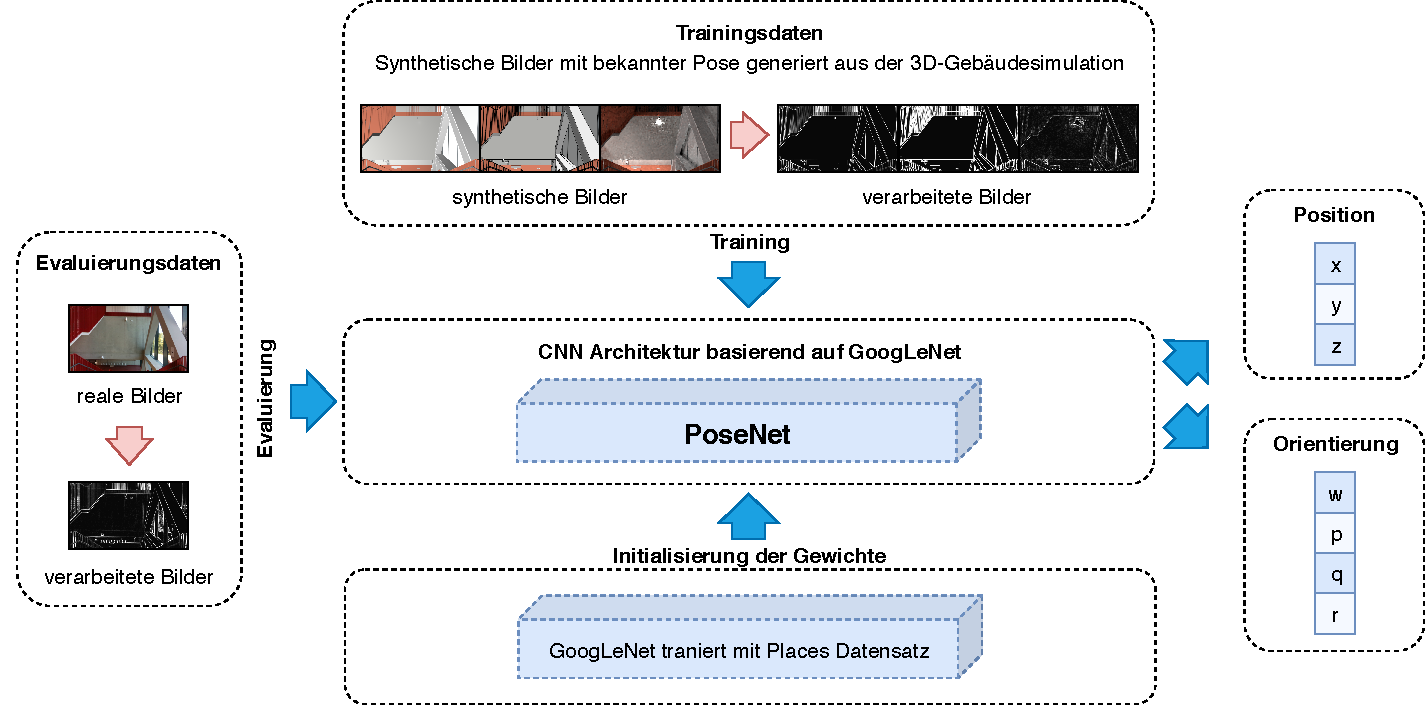
\includegraphics[width=0.85\textwidth]{images/methodik/methodik.pdf}
	\caption{Visualisierung der Methodik. Abbildung basiert auf \cite{acharyaBIMPoseNetIndoorCamera2019}.}
	\label{fig:methodik}
\end{figure}


\subsection{Erhebung der realen Daten}
\label{subsec:record_real_data}
In der Literatur wurden SfM-Methoden eingesetzt, um die Ground-Truth-Daten der realen Aufnahmen zu bestimmen \cite{kendallPoseNetConvolutionalNetwork2015, clarkVidLocDeepSpatioTemporal2017, acharyaBIMPoseNetIndoorCamera2019}. 
In der vorliegenden Arbeit wurde für die Bestimmung der Ground-Truth-Daten sowie die Aufnahme der Bilder zeitgleich zwei unterschiedliche Kameras der Intel Realsense Reihe verwendet. Eine Intel Realsense T265\footnote{\url{https://www.intelrealsense.com/tracking-camera-t265/} (abgerufen am: 18.07.2019)} wurde eingesetzt, die die relative Pose zum Ausgangspunkt mit einer Abweichung von weniger als 1\%, bei gegebener Bestkonditionen, über die SfM von zwei Fischaugenkameras (Auflösung von $848 \times 800$) und Inertial Measurement Units (\textit{IMU}) zu ermitteln verspricht. Zudem wurde eine Intel Realsense D435\footnote{ \url{https://www.intelrealsense.com/depth-camera-d435/} (abgerufen am: 18.07.2019)} eingesetzt, die eine 3D Punktwolke, ein $1280\times720$ Tiefenbild sowie ein $1920\times1080$ RGB-Bild einer Szene liefert. Die T265 wurde über die D435 montiert (siehe Abb. \ref{fig:t265_d435}), um die RGB-Bilder der D435 mit den Ground-Truth-Daten der T265 annotieren zu können.

\begin{figure}
	\centering
	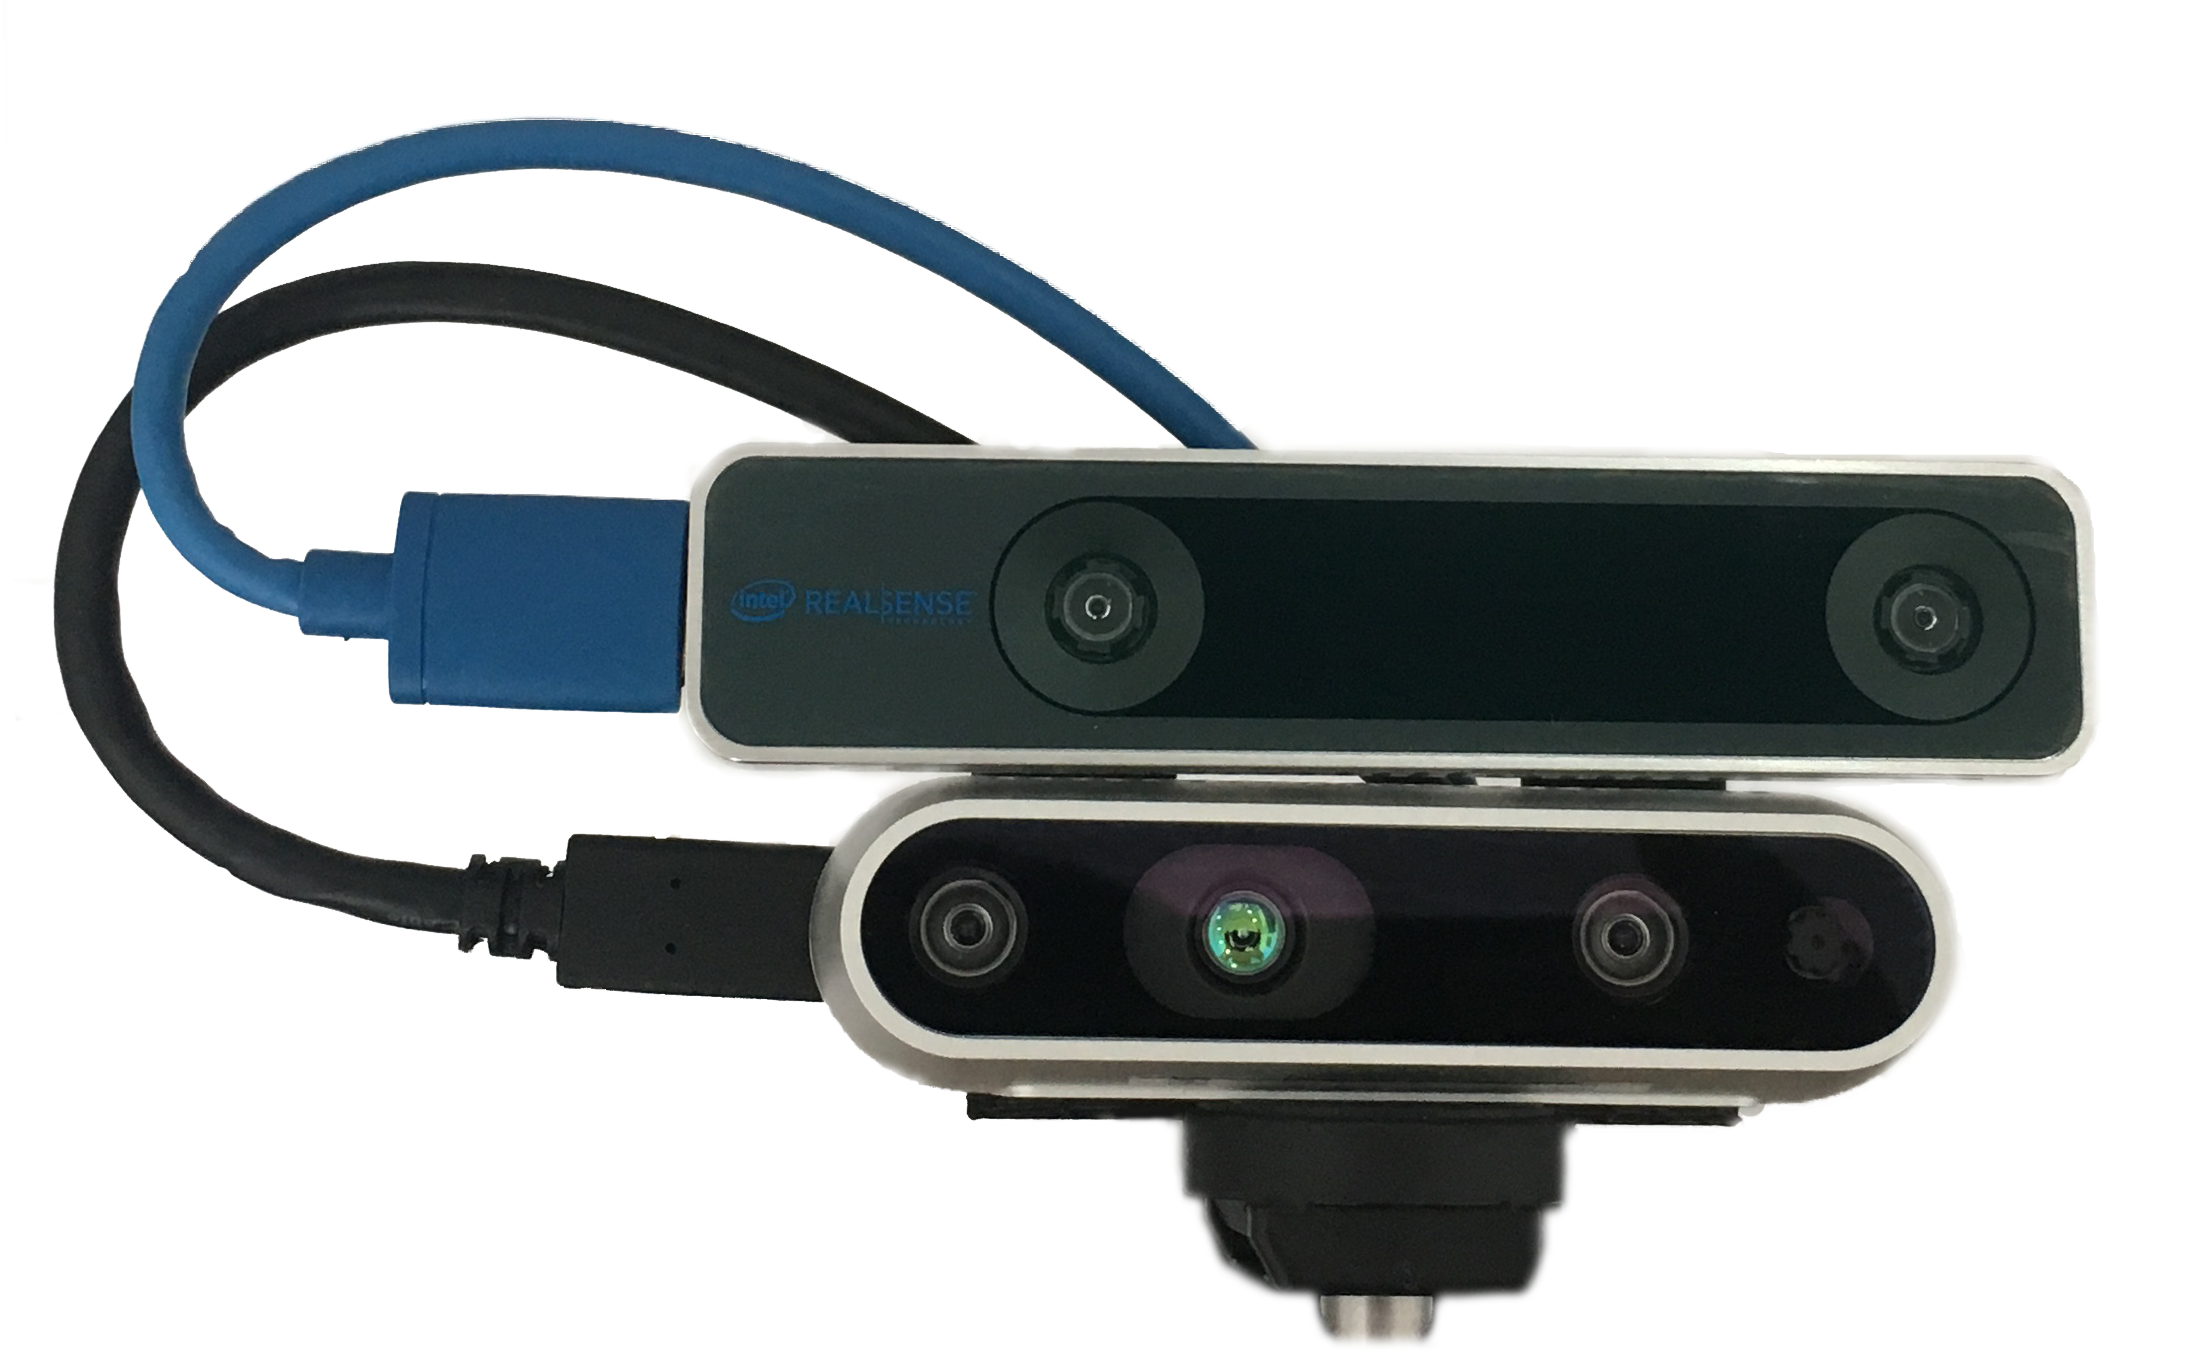
\includegraphics[width=0.5\textwidth]{images/real_dataset/t265_d435_2.png}
	\caption{Hardware für die Aufnahme der realen Daten. Die Intel Realsense T265 ist oberhalb der Intel Realsense D435 montiert.}
	\label{fig:t265_d435}
\end{figure}

In der Literatur wurden die realen Daten einer Zone grundsätzlich entlang einer Strecke aufgenommen \cite{kendallPoseNetConvolutionalNetwork2015, clarkVidLocDeepSpatioTemporal2017, acharyaBIMPoseNetIndoorCamera2019}. Daher wurden zuerst Aufnahmestrecken in den Gebäudesimulationen festgelegt und anschließend die Aufnahmen durchgeführt. Davor wurden die Ausgangspunkte der Aufnahmen zu einem Referenzpunkt in den Simulationen abgemessen und als Offset zur Bestimmung der globalen Position im Gebäude notiert.


Über das Robot Operating System\footnote{\url{https://www.ros.org/about-ros/} (abgerufen am: 18.07.2019)} (\textit{ROS}) Framework wurden die Kameras zeitgleich angesprochen und der Datenfluss der Kameras synchronisiert. Anschließend wurde der notierte Offset zur Bestimmung der absoluten Position im Gebäude zu den von der T265 berechneten, zur Ausgangspunkt relativen, Posen addiert. Somit beinhaltet jeder erhobene Datensatz ein Bild je Fischaugenkamera, ein Tiefenbild, ein RGB-Bild, eine 3D Punktwolke und die dazugehörige absolute Pose im Gebäude pro Frame. Für die vorliegende Arbeit waren nur die Pose-Daten der T265 sowie die RGB-Bilder der D435 relevant, da PoseNet ausschließlich RGB-Bilder mit annotiertem Kamerapose benötigt. Abbildung \ref{fig:dataset} visualisiert ein Datensatzexemplar für einen Frame.

Aus Zeitgründen konnten die Bestkonditionen für die T265 nicht hergestellt werden, sodass die von der T265 berechneten Posen eine Abweichung (\textit{Drift}) bis zur 5\% (vgl. Abb. \ref{fig:trajectories}) aufweisen. Da in der vorliegenden Arbeit die realen Daten zur Evaluierung eingesetzt wurden, allenfalls für die Bestimmtung eines Hyperparameters zwecks der Evaluierung mit den realen Daten trainiert wurde, sowie die Akkuratesse im Meterbereich für eine Beobachtung ausreichen sollte, wurde die Abweichung der Posen nicht korrigiert.


\begin{figure}
	\centering
	\begin{subfigure}[t]{0.3\linewidth}
		\centering
		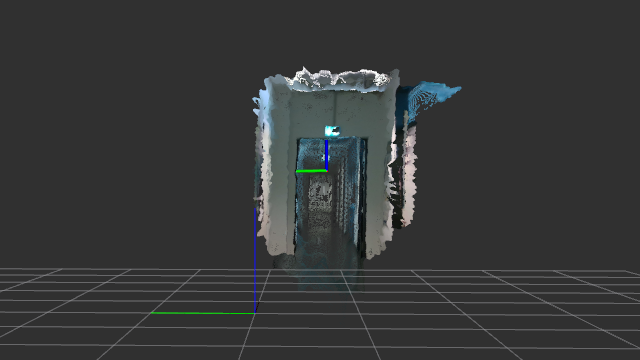
\includegraphics[width=\linewidth]{images/real_dataset/pointcloud3.png}
		\caption{Odometrie  (T265) + \\ 3D Punktwolke (D435)}
		\label{subfig:odom1}
	\end{subfigure}
	\hfill
	\begin{subfigure}[t]{0.3\linewidth}
		\centering
		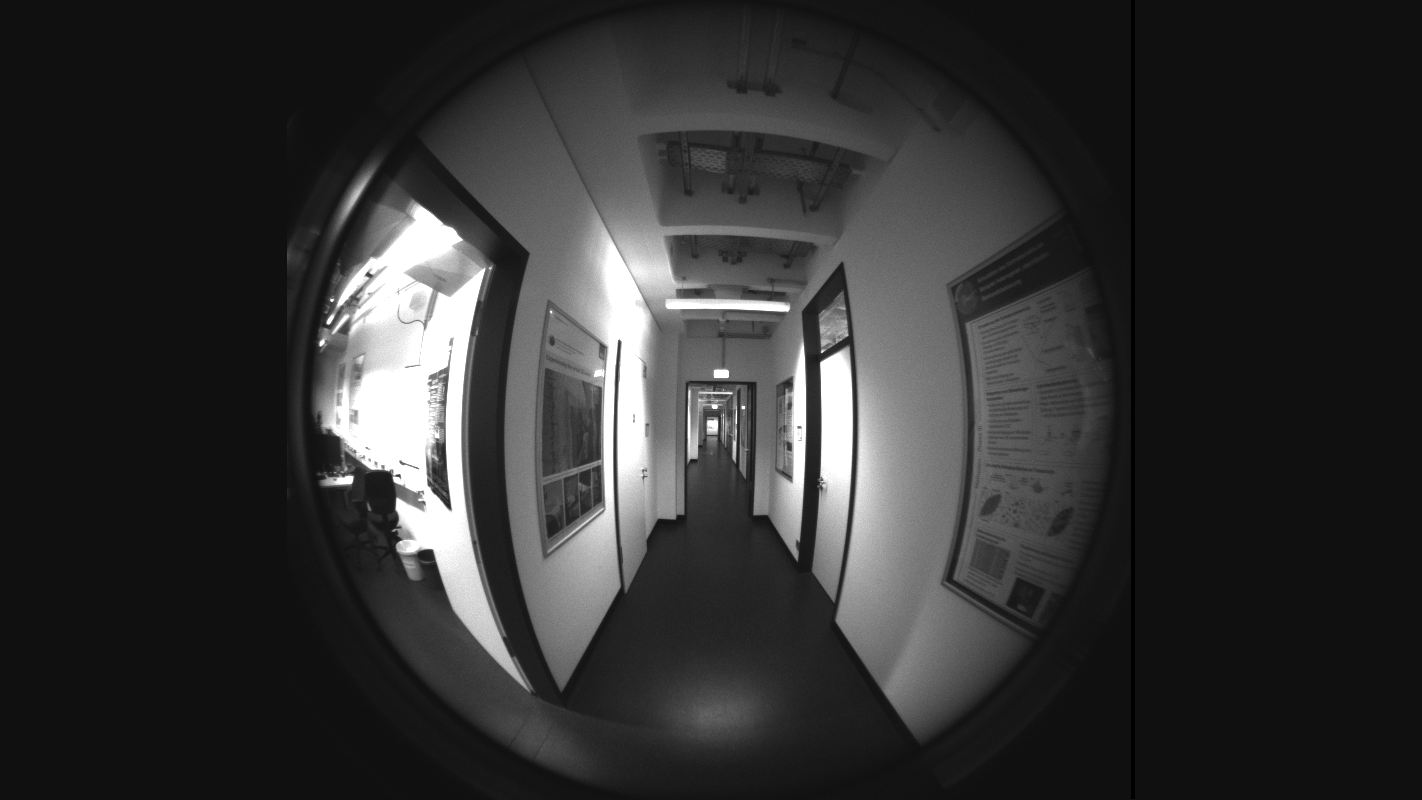
\includegraphics[width=\linewidth]{images/real_dataset/f1_frame000005.png}
		\caption{Fischaugenkamera 1 \\ (T265)}
		\label{subfig:fisheye1}
	\end{subfigure}
	\hfill
	\begin{subfigure}[t]{0.3\linewidth}
		\centering
		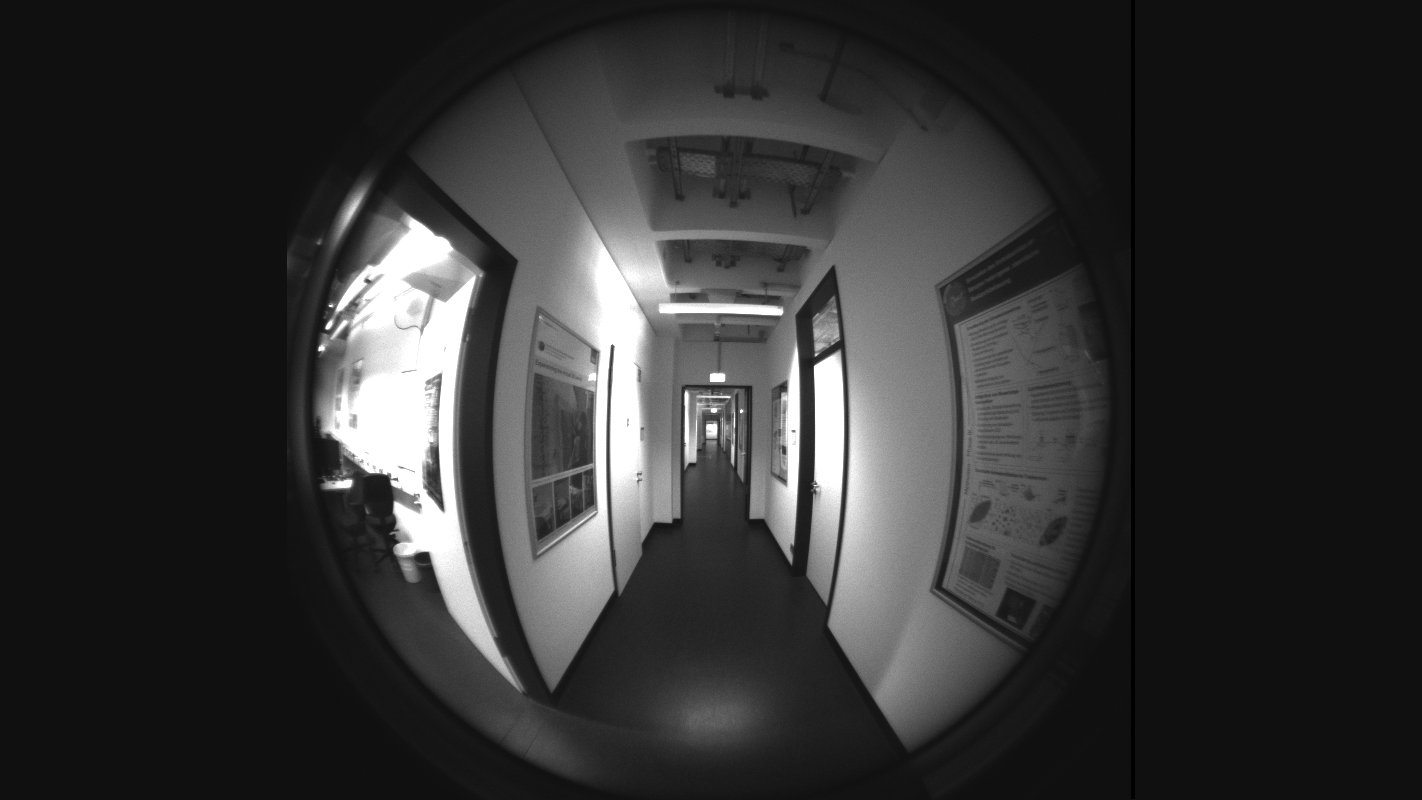
\includegraphics[width=\linewidth]{images/real_dataset/f2_frame000005.png}
		\caption{Fischaugenkamera 2 \\ (T265)}
		\label{subfig:fisheye2}
	\end{subfigure}
	\hfill \medskip
	\begin{subfigure}[t]{0.3\linewidth}
		\centering
		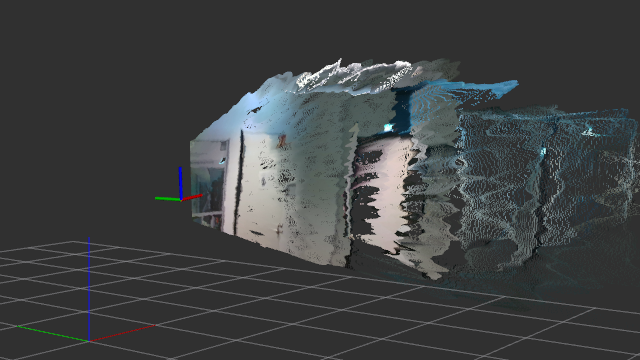
\includegraphics[width=\linewidth]{images/real_dataset/pointcloud1.png}
		\caption{Odometrie  (T265) + \\ 3D Punktwolke (D435)}
		\label{subfig:odom2}
	\end{subfigure}
	\hfill
	\begin{subfigure}[t]{0.3\linewidth}
		\centering
		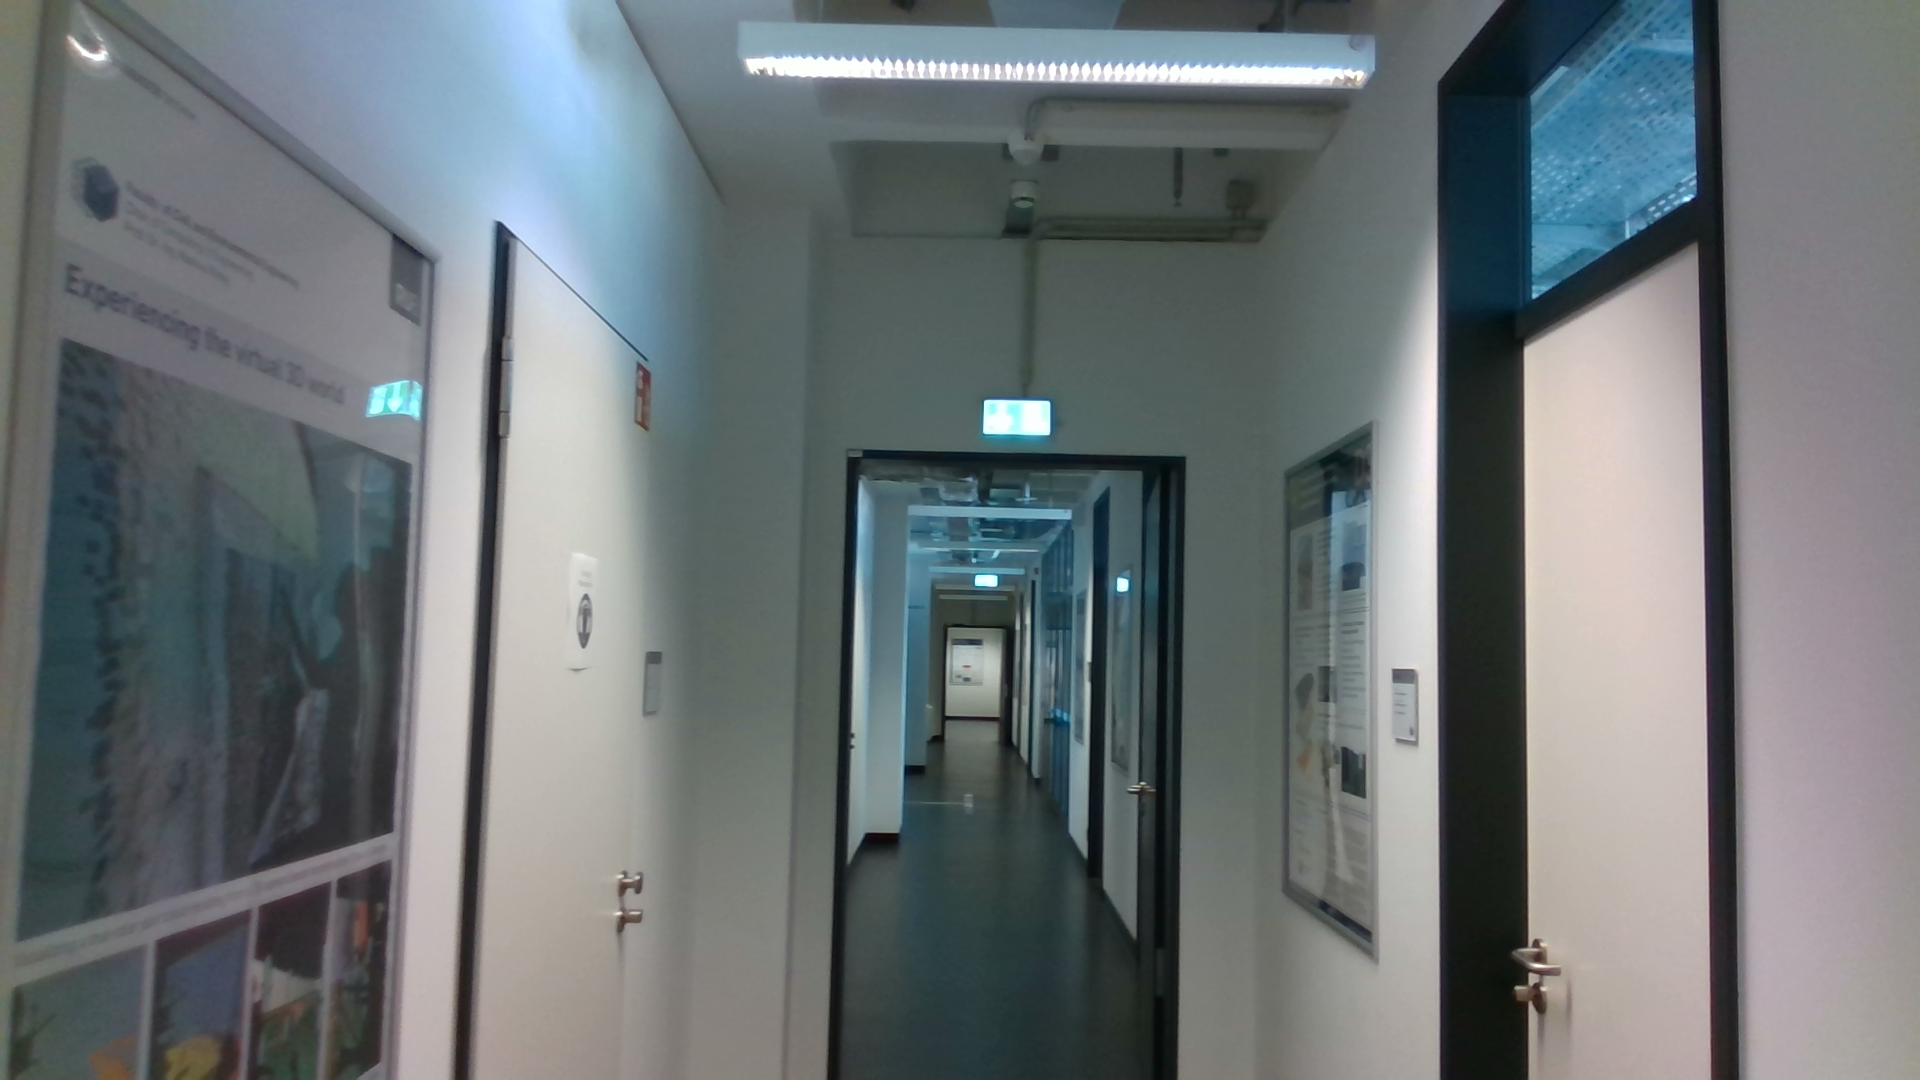
\includegraphics[width=\linewidth]{images/real_dataset/dc_frame000005.png}
		\caption{RGB-Bild \\ (D435) \hspace*{2cm}}
		\label{subfig:rgb-image}
	\end{subfigure}
	\hfill
	\begin{subfigure}[t]{0.3\linewidth}
		\centering
		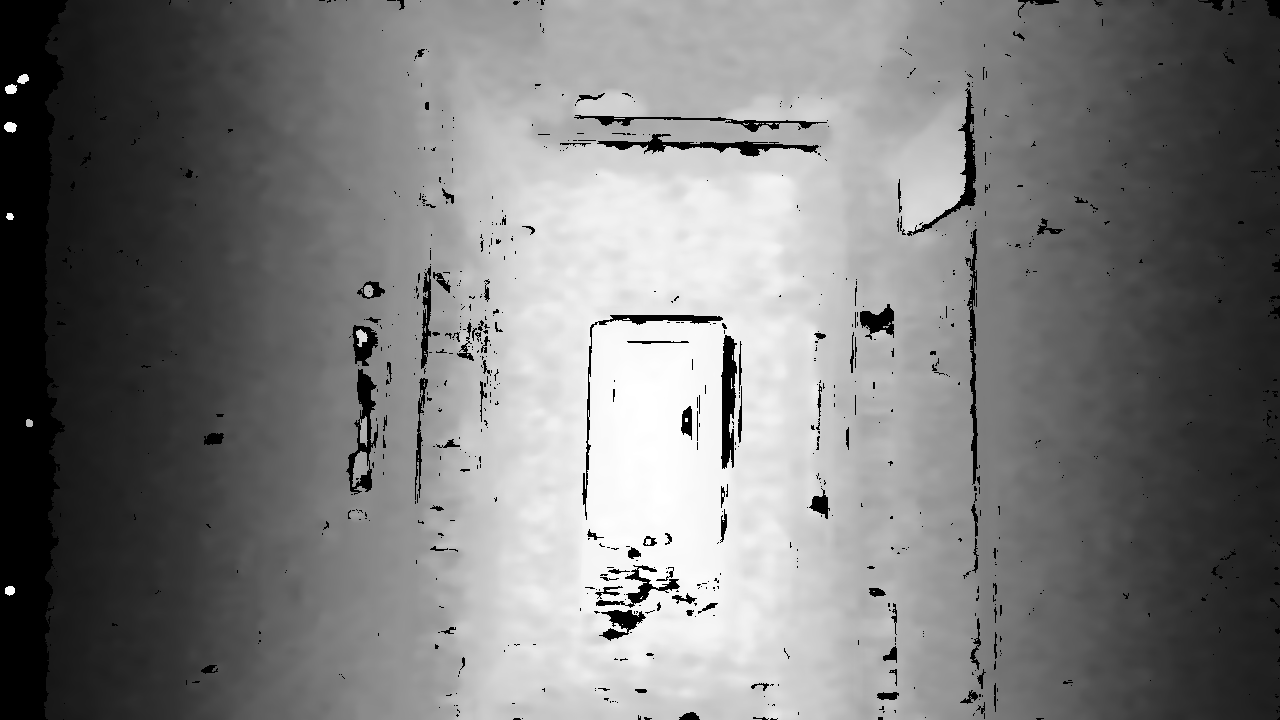
\includegraphics[width=\linewidth]{images/real_dataset/dt_frame000005.png}
		\caption{Tiefenbild \\ (D435) \hspace*{2cm}}
		\label{subfig:depth-image}
	\end{subfigure}
	\caption{Datensatz pro Frame. \subref{subfig:odom1}  und \subref{subfig:odom2} visualisieren in unterschiedlichen Prespektiven die von der T265 ermittelte Odometrie und die von der D435 erhaltenen 3D Punktwolke. \subref{subfig:fisheye1} und \subref{subfig:fisheye2} sind die von der T265 aufgenommenen Fischaugenbilder. \subref{subfig:rgb-image} ist das RGB-Bild der D435 und \subref{subfig:depth-image} das dazugehörige Tiefenbild. }
	\label{fig:dataset}
\end{figure}

\subsection{Generierung der synthetischen Daten}
\label{subsec:generate_synth_images}
Für die Generierung der synthetischen Daten wurden die 3D-Gebäudemodelle  aus dem BIM der Gebäuden entnommen. Die 3D-Gebäudemodelle wurden in Blender\footnote{\url{https://www.blender.org/about/} (aufgerufen am: 20.07.2019)} in der derzeitig aktuellen Version 2.79b simuliert. Die intrinsischen Daten der D435 RGB-Kamera wurden auf die virtuellen Kameras übertragen. Aus Gründen der Performance wurde die Auflösung der synthetischen Bilder von $1920\times1080$ auf  $960\times540$ halbiert.

Die Strecken der realen Aufnahmen wurden in den Simulationen Konsistenz halber auf einer konstanten Höhe von 1.70$m$ bestmöglich schwankungslos imitiert. Eine exakte Imitation der Aufnahmestrecke der realen Daten war wegen des Abdriftens der von der T265 berechneten Ground-Truth-Daten nicht möglich (siehe Abschnitt \ref{subsec:record_real_data}).

In Anlehnung an \citet{acharyaBIMPoseNetIndoorCamera2019} wurde entlang der Strecke in 0.05$m$ Intervallen und mit einer $\pm$10° Neigung in je y- und z-Achse Bilder mit korrespondierenden Ground-Truth-Daten aufgenommen, um die Varianz der realen Daten abzudecken. Abbildung \ref{fig:dataset_variation} illustriert die Variationen der Pose pro Stützpunkt auf einer Strecke.


\begin{figure}
	\centering
	\begin{subfigure}[t]{0.18\linewidth}
		\centering
		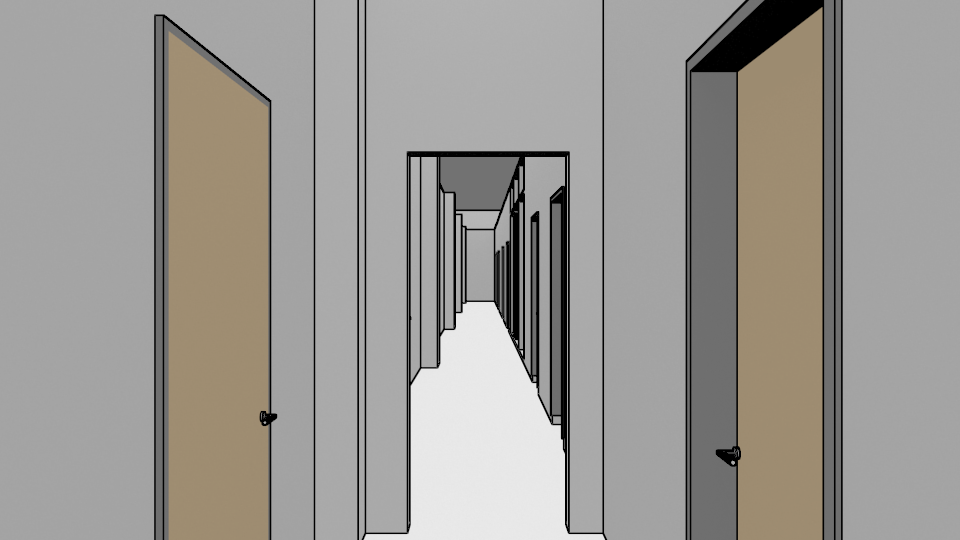
\includegraphics[width=\linewidth]{images/syn_dataset/00023.png}
		\caption{Orginal Pose \vspace{\fill}}
		\label{subfig:iz0_y0}
	\end{subfigure}
	\hfill 
	\begin{subfigure}[t]{0.18\linewidth}
		\centering
		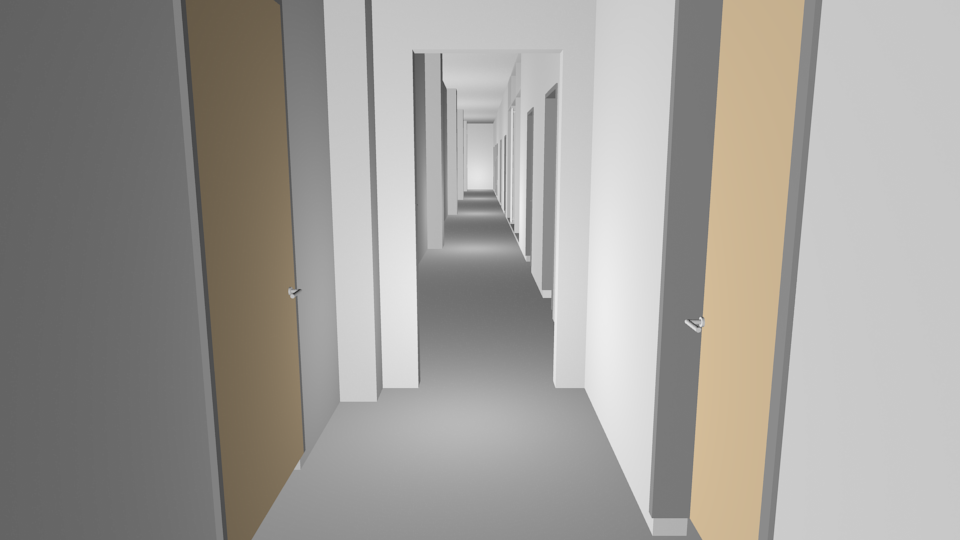
\includegraphics[width=\linewidth]{images/syn_dataset/00021.png}
		\caption{-10° um die y-Achse}
		\label{subfig:iz0_y-10}
	\end{subfigure}
	\hfill
	\begin{subfigure}[t]{0.18\linewidth}
		\centering
		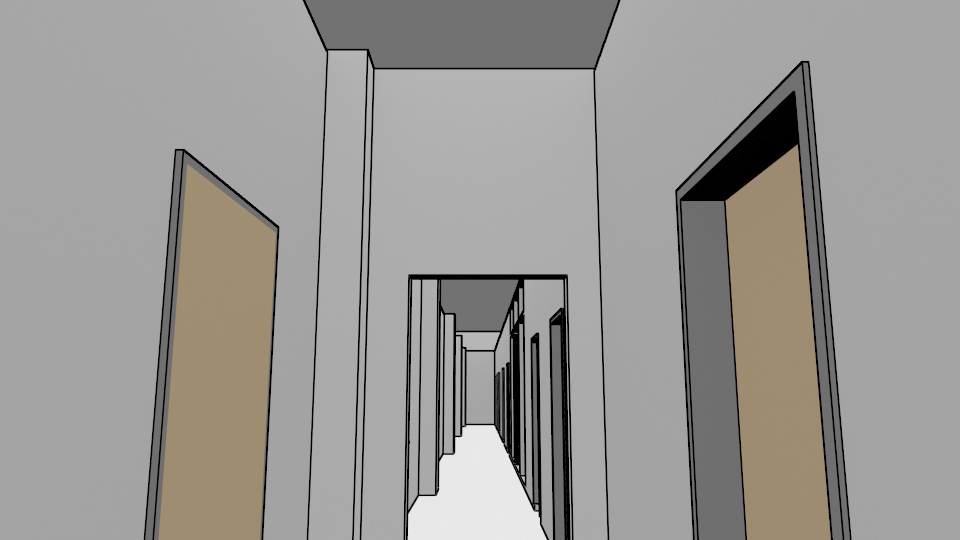
\includegraphics[width=\linewidth]{images/syn_dataset/00020.png}
		\caption{+10° um die y-Achse}
		\label{subfig:iz0_y+10}
	\end{subfigure}
	\hfill
	\begin{subfigure}[t]{0.18\linewidth}
		\centering
		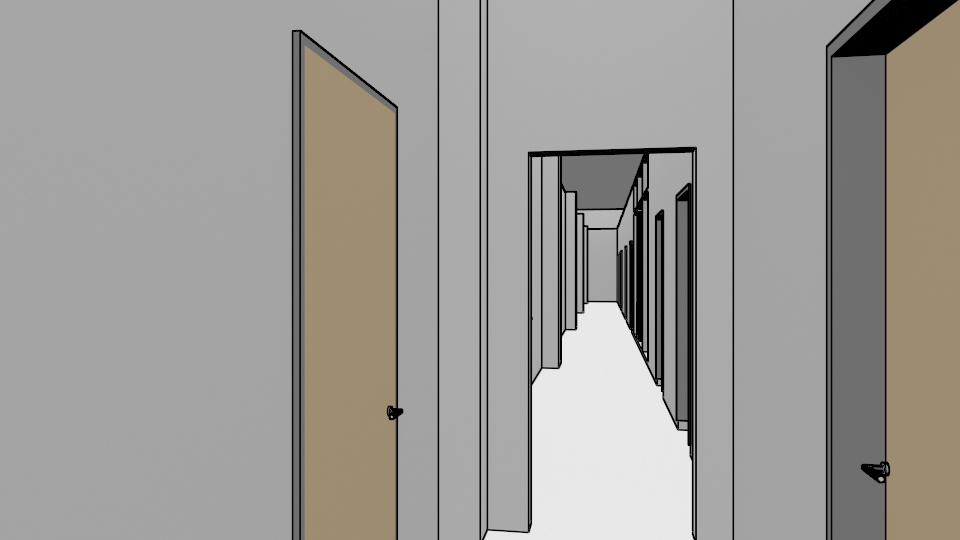
\includegraphics[width=\linewidth]{images/syn_dataset/00024.png}
		\caption{-10° um die z-Achse}
		\label{subfig:iz-10_y0}
	\end{subfigure}
	\hfill
	\begin{subfigure}[t]{0.18\linewidth}
		\centering
		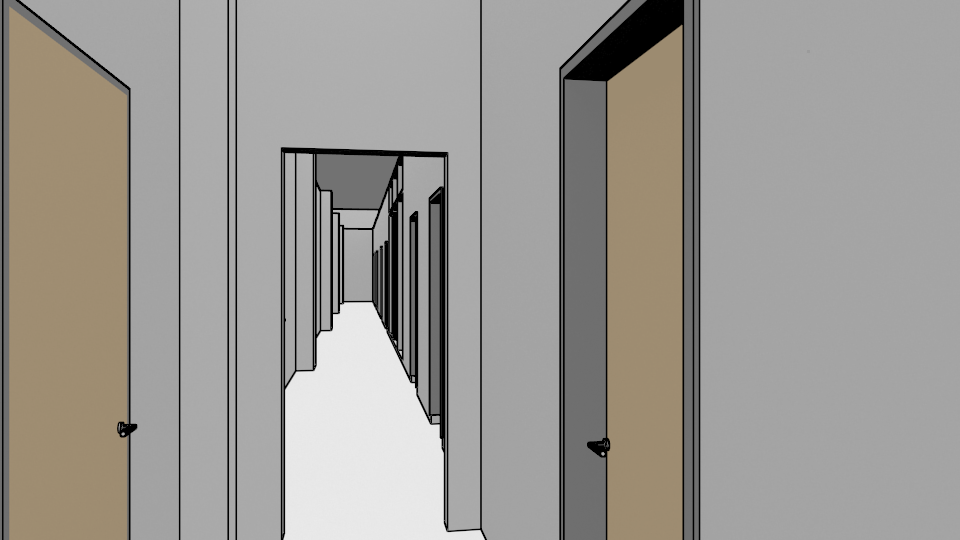
\includegraphics[width=\linewidth]{images/syn_dataset/00022.png}
		\caption{+10° um die z-Achse}
		\label{subfig:iz+10_y0}
	\end{subfigure}
	\caption{Variation der Pose pro Stützpunkt auf einer Strecke.}
	\label{fig:dataset_variation}
\end{figure}

Insgesamt wurden drei synthetische Datensätze je Strecke erzeugt, gleicherweise wie die synthetischen Datensätze von \citet{acharyaBIMPoseNetIndoorCamera2019}, die sich in der Beschaffenheit von karikaturistische Darstellung, zu synthetischen Kantenbilder, hin über zu fotorealistische Darstellung unterscheiden (siehe Abb. \ref{fig:dataset_preprocess}). Bei der Generierung der karikaturistischen und fotorealistischen Datensätzen wurde die Beleuchtung aus einem Netz von Punktlichtquellen nachgestellt, um die Lichteffekte realitätsnäher zu simulieren.
Für die Erzeugung der synthetischen Kantenbilder wurden die Kanten der 3D-Objekte über Blender markant sichtbar konfiguriert und eine homogene Beleuchtung verschaffen, damit die Kanten hervorstechen und unberührt von Beleuchtungseffekte bleiben (vgl. Abb. \ref{fig:dataset}). 

 Die karikaturistische und fotorealistische Datensätze unterscheiden sich ausschließlich in den Render-Engines. Blender 2.79b bietet die Render-Engines \textit{Blender-Internal} und \textit{Blender-Cycles}. Während die Blender-Internal Engine beim Rendern die Berechnung der Lichtstrahlen abkürzt, versucht die Blender-Cycles Engine über Raytracing-Algorithmen das Verhalten des Lichtes mit ihren physikalischen Eigenschaften zu simulieren. Daher wurden die karikaturistischen Datensätze sowie die Kantenbilder über die Render-Engine \textit{Blender-Internal} und der fotorealistischer Datensatz über die \textit{Blender-Cycles} Engine generiert.

\subsection{Verarbeitung der Daten}
Die vorliegende Arbeit versucht das PoseNet Modell mit den Gradientenbilder der synthetischen Daten zu trainieren und mit den Gradietenbilder der realen Daten zu evaluiert. Daher wurde nach der Erhebung der realen Bilder (siehe Abschnitt \ref{subsec:record_real_data}) und Generierung der synthetischen Bilder (siehe Abschnitt \ref{subsec:generate_synth_images}) diese in ihre Gradientenbilder verarbeitet. Die realen Bilder wurden vor der Verarbeitung in Gradientenbilder auf die Größe $960 \times 540$ der synthetischen Bilder verkleinert, um einerseits eine einheitliche Auflösung der Bilder zu verschaffen und andererseits unscharfe Kanten, bedingt durch Bewegung, im Bild zu einer schärferen Kante zusammenzuführen, da schärfere Kanten im Vergleich zu unscharfen Kanten im Bild eine deutlichere Kontur im Gradientenbild aufweisen.

Die künstliche Beleuchtung in den Gebäudesimulationen führte bei den Gradientenbildern der karikaturistischen Daten zu Artefakten (vgl. Abb. \ref
{fig:treshold}). Diese Artefakten befanden sich im niedrigen Wertebereich des Gradientenbildes. Daher wurde für die Unterdrückung der Artefakten zusätzlich ein Schwellenwertverfahren angewendet, indem die Pixelwerte eines Gradientenbildes unter einer gewissen Schwelle auf ein Mindestwert gesetzt werden. Es wurde iterativ nach einem Minimum der Pixelwerte gesucht, sodass die von den Artefakten betroffenen Stellen eine homogene Fläche im Bild darstellen. Der Wert 8 stellte sich als geeignete Schwelle für die Gradientenbilder heraus und wurde als Minimum für die Pixelwerte festgelegt, sodass die Pixelwerte der Gradientenbilder im Wertebereich von $[8,255]$ liegen. Da es sich bei dem Pixelwert 8 um einen kleinen Wert handelt, wurde Konsistenz halber dieses Verfahren bei allen Datensatztypen angewendet. Abbildung \ref{fig:dataset_preprocess} visualisiert von jedem Datensatztyp ein Beispiel und die dazugehörigen Gradientenbilder.


\begin{figure}
	\centering
	\begin{tikzpicture}[zoomboxarray, 
	connect zoomboxes,
	zoomboxarray columns=2,
	zoomboxarray rows=1,
	zoombox paths/.append style={thick, orange},
	figurename=notresh]
	\node [image node] { 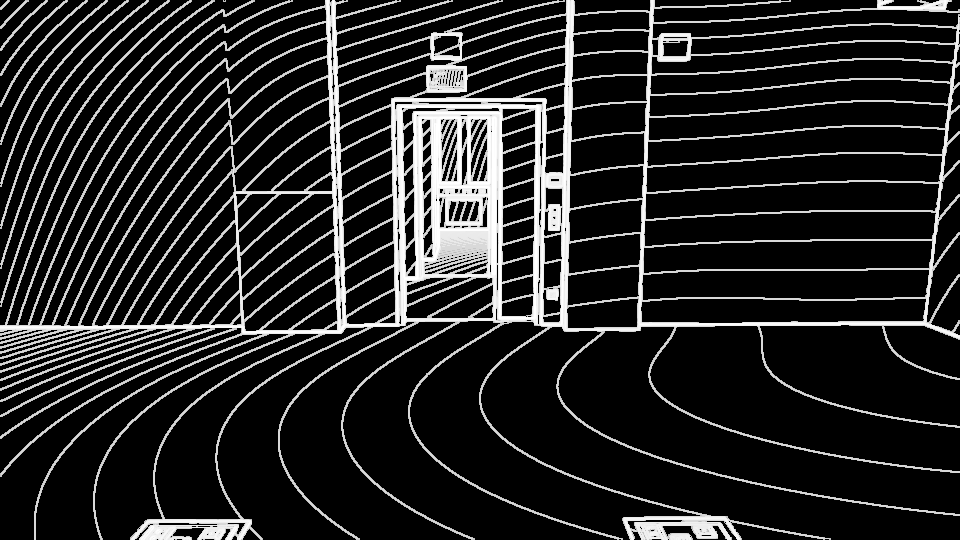
\includegraphics[width=0.24\textwidth]{images/treshold/0_tresh_binared.png} };
	\zoombox[magnification=10]{0.15,0.8}
	\zoombox[magnification=10]{0.5,0.25}
	\end{tikzpicture}
	\begin{tikzpicture}[zoomboxarray, 
	connect zoomboxes,
	zoomboxarray columns=2,
	zoomboxarray rows=1,
	zoombox paths/.append style={thick, orange},
	figurename=treshed]
	\node [image node] { 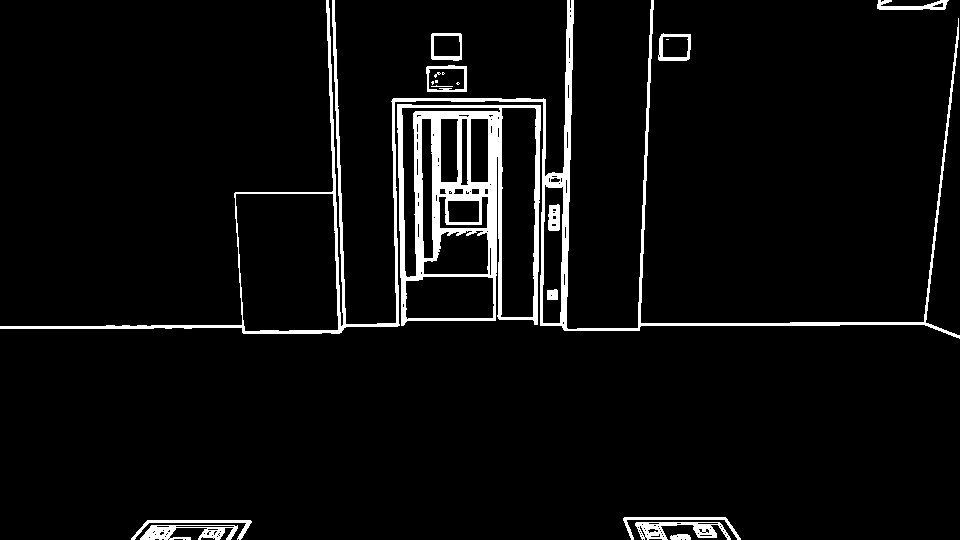
\includegraphics[width=0.24\textwidth]{images/treshold/8_tresh_binared.png} };
	\zoombox[magnification=10]{0.15,0.8}
	\zoombox[magnification=10]{0.5,0.25}
	\end{tikzpicture}
	\caption{Darstellung der durch die künstliche Beleuchtung entstehenden Artefakten in den Gradientenbilder der karikaturistischen Daten. Für eine bessere Visualisierung der Artefakten wurden die Gradientenbild binarisiert. \subref{notresh-image} ist ein Gradientenbild ohne Anwendung eines Schwellenwertverfahrens. \subref{treshed-image} ist ein Gradientenbild mit Anwendung eines Schwellenwertverfahrens.}
	\label{fig:treshold}
\end{figure}


\begin{figure}
	\centering
	\begin{subfigure}[t]{0.24\linewidth}
		\centering
		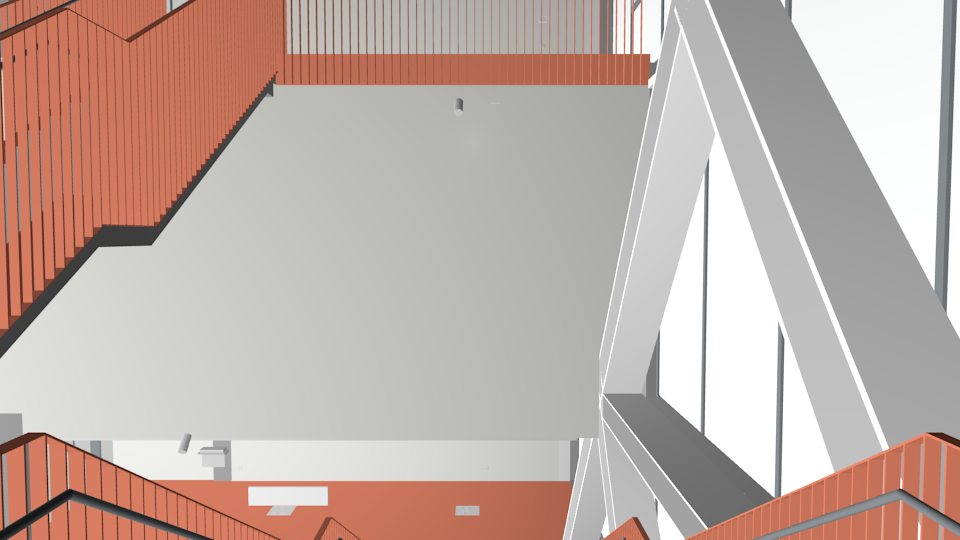
\includegraphics[width=\linewidth]{images/syn_dataset/b00188.png}
		\caption{karikaturistische Simulation}
		\label{subfig:cartoonish}
	\end{subfigure}
	\hfill
	\begin{subfigure}[t]{0.24\linewidth}
		\centering
		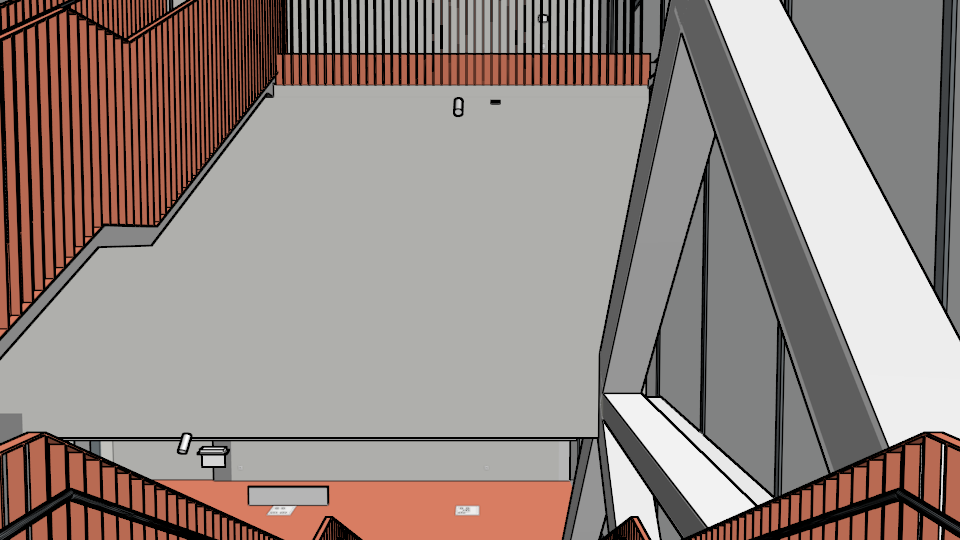
\includegraphics[width=\linewidth]{images/syn_dataset/e00188.png}
		\caption{synthetisches \hspace{1cm} Kantenbild}
		\label{subfig:edge}
	\end{subfigure}
	\hfill
	\begin{subfigure}[t]{0.24\linewidth}
		\centering
		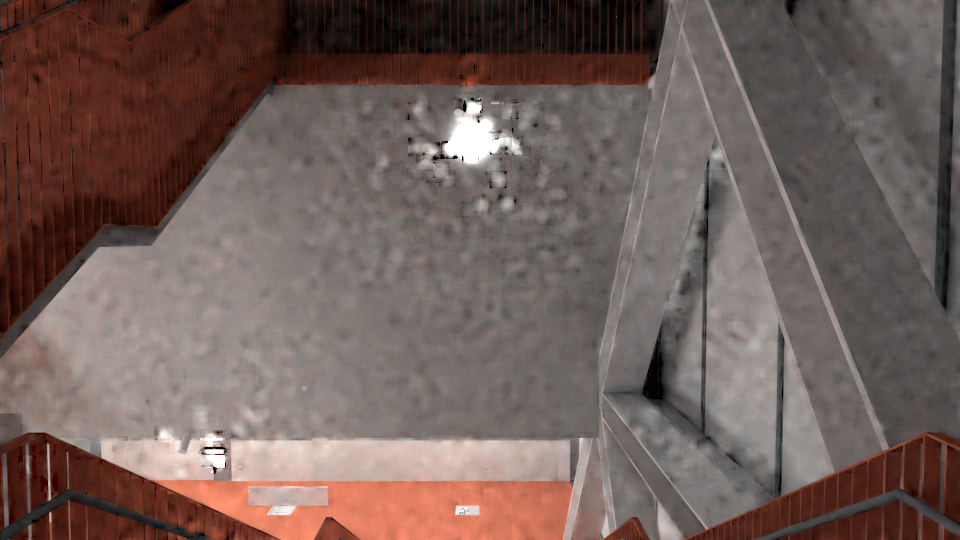
\includegraphics[width=\linewidth]{images/syn_dataset/c00188.png}
		\caption{fotorealistische \hspace{1cm} Simulation}
		\label{subfig:photorealistic}
	\end{subfigure}
	\hfill 
	\begin{subfigure}[t]{0.24\linewidth}
		\centering
		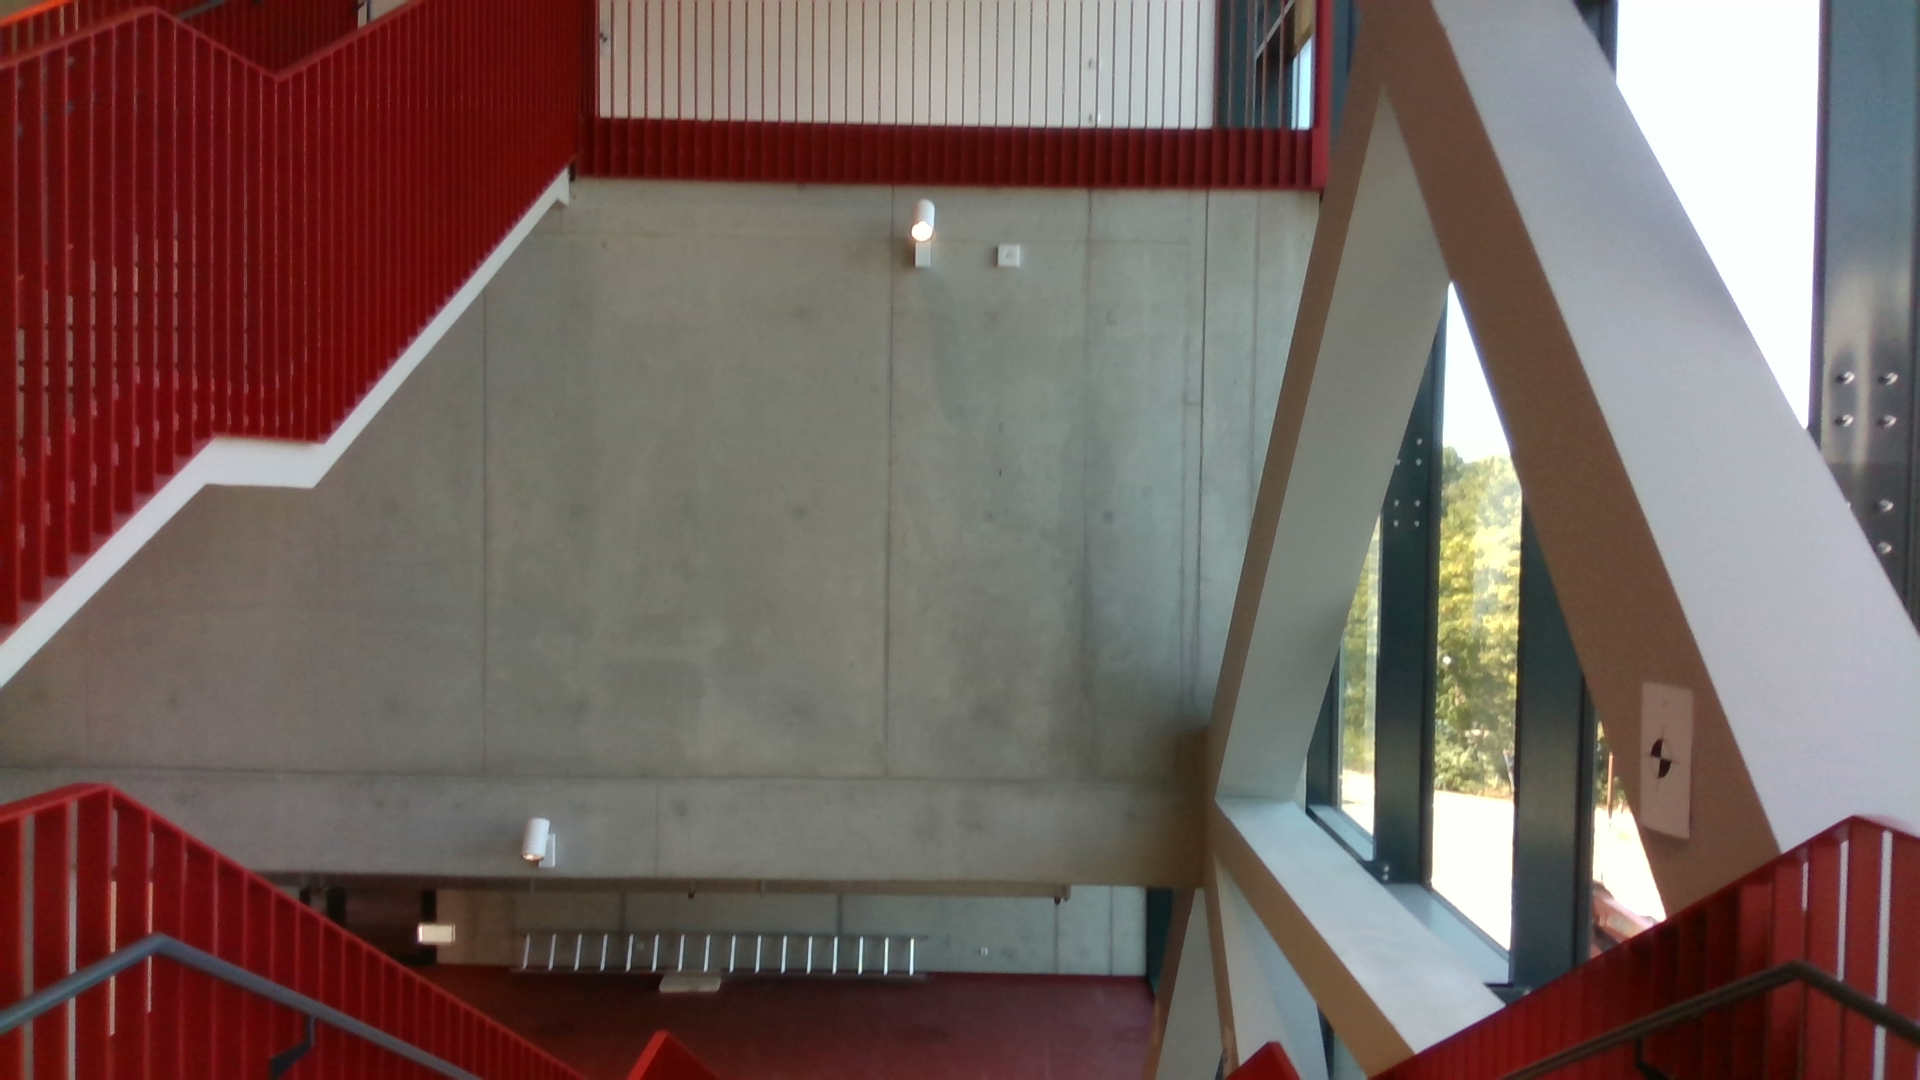
\includegraphics[width=\linewidth]{images/syn_dataset/r000089.png}
		\caption{reale Aufnahme \hspace{2cm}}
		\label{subfig:real}
	\end{subfigure}
	\hfill 
	\begin{subfigure}[t]{0.24\linewidth}
		\centering
		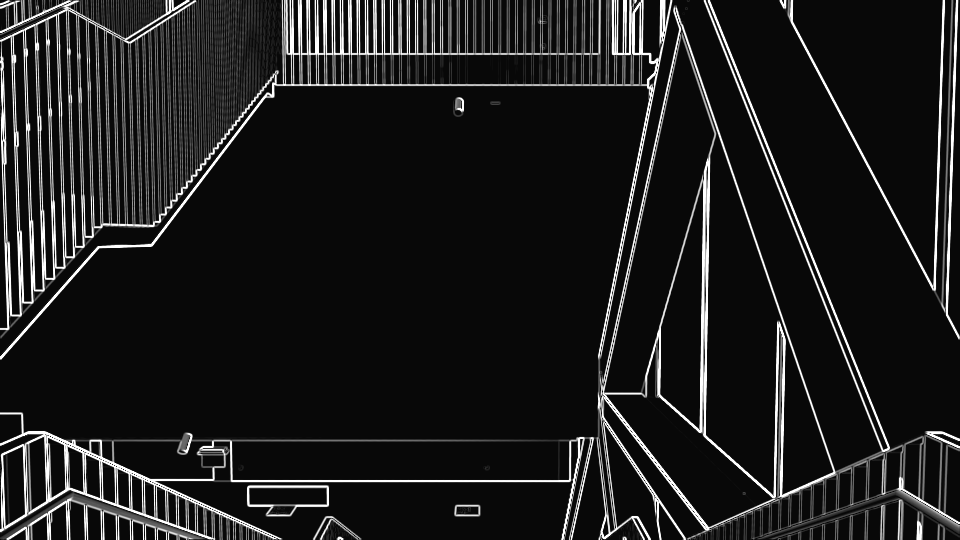
\includegraphics[width=\linewidth]{images/syn_dataset/bg00188.png}
		\caption{Gradientenbild  \hspace{1cm} von \subref{subfig:cartoonish}}
	\end{subfigure}
	\hfill
	\begin{subfigure}[t]{0.24\linewidth}
		\centering
		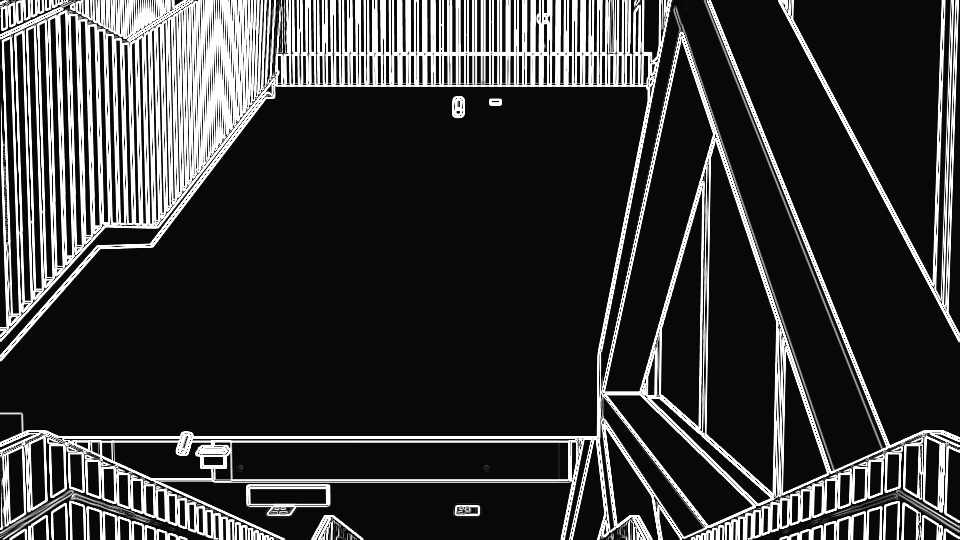
\includegraphics[width=\linewidth]{images/syn_dataset/eg00188.png}
		\caption{Gradientenbild  \hspace{1cm} von \subref{subfig:edge}}
	\end{subfigure}
	\hfill
	\begin{subfigure}[t]{0.24\linewidth}
		\centering
		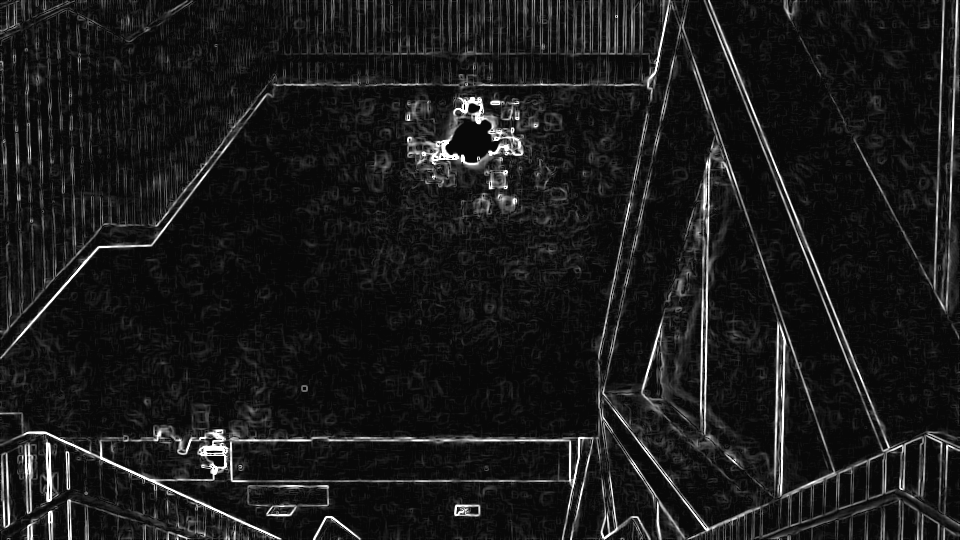
\includegraphics[width=\linewidth]{images/syn_dataset/cg00188.png}
		\caption{Gradientenbild  \hspace{1cm} von \subref{subfig:photorealistic}}
	\end{subfigure}
	\hfill
	\begin{subfigure}[t]{0.24\linewidth}
		\centering
		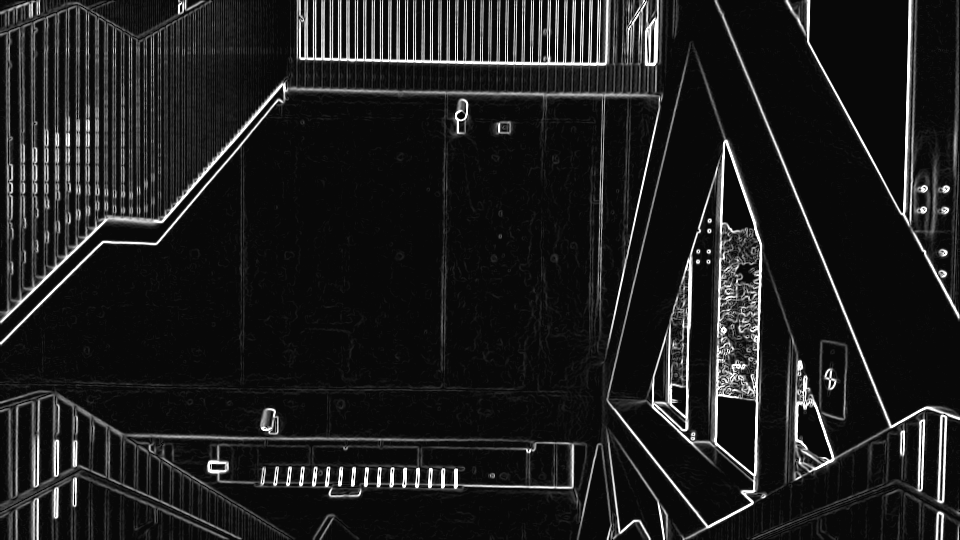
\includegraphics[width=\linewidth]{images/syn_dataset/rg000089.png}
		\caption{Gradientenbild  \hspace{1cm} von \subref{subfig:real}}
	\end{subfigure}
	\hfill
	\caption{Beispielhafte Bilder für jeden Datensatztyp und die dazu korrespondierenden Gradientenbilden. Die Daten sind aus dem \textit{IC-loop} Datensatz.}
	\label{fig:dataset_preprocess}
\end{figure}

\cleardoublepage



\subsection{Datensätze}
\label{subsec:datasets}
Diese Arbeit versucht den Ansatz von \citet{acharyaBIMPoseNetIndoorCamera2019} auf längeren Strecken in größeren Gebäudesimulation zu untersuchen. Der Datensatz von \citet{acharyaBIMPoseNetIndoorCamera2019} erstreckt sich über ca. 18$m$ in einem ca. $20m \times 5m$ großen Korridor auf einer Etagenebene und die Aufnahme verlief überwiegen in einer Richtung (vgl. Abb. \ref{fig:acharya_traj}). Daher wurden längere Aufnahmestrecken festgelegt, die einerseits in mehrere Richtungen verlaufen und andererseits sich auf mehreren Etagenebenen erstrecken. Zudem wurden die Aufnahmestrecken so festgelegt, dass die Aufnahmestrecken Herausforderungen wie z.B. das \textit{Loop-Closure}- bzw. \textit{Perceptual-Aliasing}-Problem berücksichtigen.

\begin{figure}
	\centering
	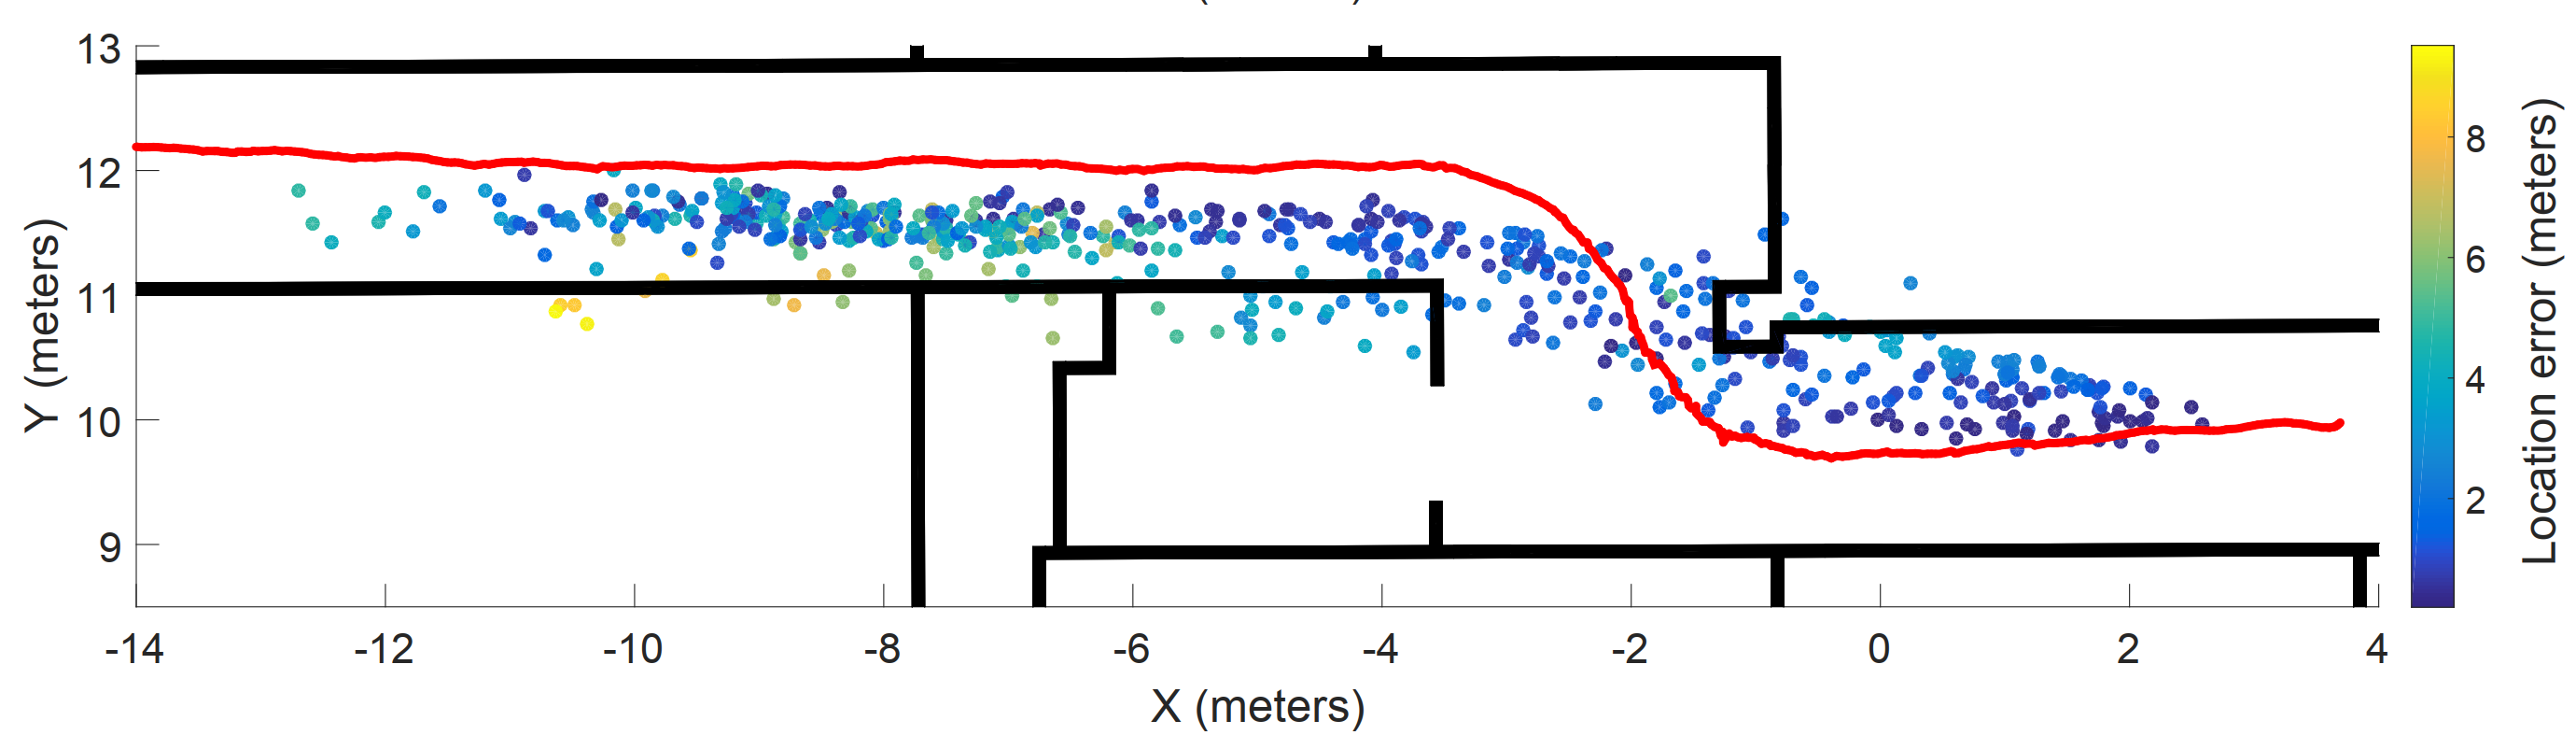
\includegraphics[width=1.0\textwidth]{images/trajectories/acharya_traj.png}
	\caption{Darstellung des Lokalisierungsergebnisses von \citet{acharyaBIMPoseNetIndoorCamera2019}, die durch das Trainieren mit den synthetischen Kantenbildern und der anschließenden Evaluierung mit den Gradientenbilder der realen Daten resultierte. Die Aufnahmestrecke der realen Daten ist in Rot dargestellt. Die Aufnahme auf der Strecke verlief von rechts nach links. Entnommen aus \cite{acharyaBIMPoseNetIndoorCamera2019}.}
	\label{fig:acharya_traj}
\end{figure}



In dieser Arbeit wurden aus zwei unterschiedlichen Gebäuden Daten erhoben bzw. synthetische Daten aus den Gebäudesimulationen generiert. Zuerst wurde ein Datensatz aus der nördlichen Hälfte des 6. Stockwerkes des IC-Gebäudes Ruhr-Universität Bochum (\textit{IC}) erhoben. Anschließend wurden drei Datensätzen im Seminargebäude Hochschule Bochum (\textit{HS}) erhoben. Die Gebäude unterscheiden sich im Detail der Simulationen (vgl.  Abb. \ref{fig:difference_3d}). Die Simulation vom IC enthält sehr wenige Objekte wie z.B. Türen und Wände. Im Gegensatz dazu enthält die Simulation vom HS mehr Objekte wie z.B. die Objekte der technischen Gebäudeausrüstung.

Die ca. $115m$ lange Strecke im ersten Datensatz, bezeichnet als \textit{IC-loop}, bildet eine geschlossene Schleife in einem $50m \times 11m \times 3.5m$ Bereich der IC. Die $65m$ lange Strecke im \textit{HS-gamma} Datensatz einhält in der Mitte eine Schleife und übergeht zu einem optisch ähnlichen Flur wie der Ausgangsflur in einem Bereich von ca. $54m \times 10m \times 3m$ der HS. Im Datensatz \textit{HS-stairs-up} wird eine Treppe im HS aufwärts bestiegen und im Datensatz \textit{HS-stairs-down} dieselbe Treppe abgestiegen. Die Strecken auf den Treppen sind ca. $32m$ lang und befindet sich in einer ca. $12m \times 12m \times 12m$ Teilzone von HS.
Tabelle \ref{tab:dataset_metrics} listet die approximierten metrischen Eigenschaften der Datensätze auf. 
Die variierende Länge der Strecken führt in den Datensätzen zu Mengenunterschiede bei den realen sowie synthetischen Daten. Tabelle \ref{tab:datasets} stellt die Datenmenge der Datensätzen dar.
Abbildung \ref{fig:trajectories} illustriert die Strecken der Datensätze. 
\begin{figure}
	\centering
	\begin{subfigure}[t]{0.48\linewidth}
		\centering
		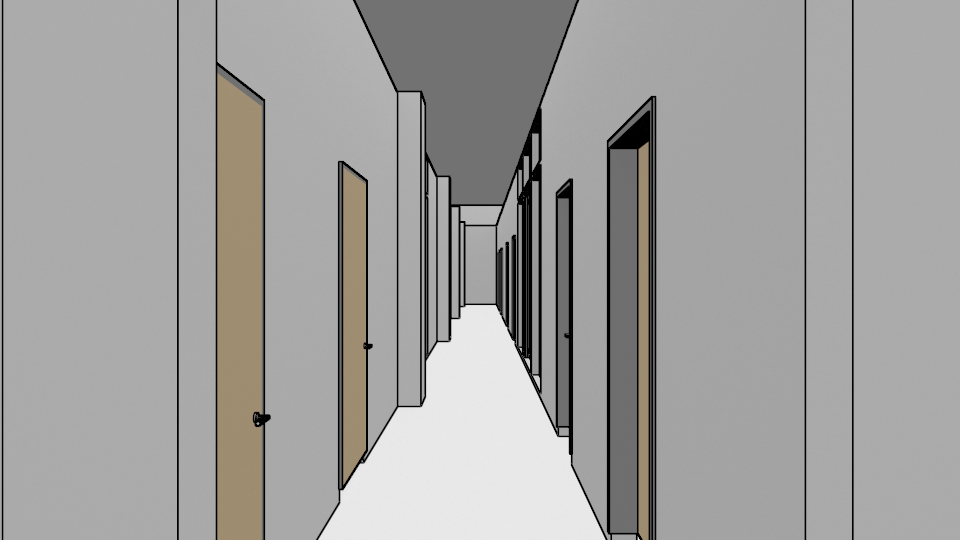
\includegraphics[width=\linewidth]{images/syn_dataset/ic00343.png}
		\caption{IC Simulation}
		\label{subfig:ic_syn_example}
	\end{subfigure}
	\hfill
	\begin{subfigure}[t]{0.48\linewidth}
		\centering
		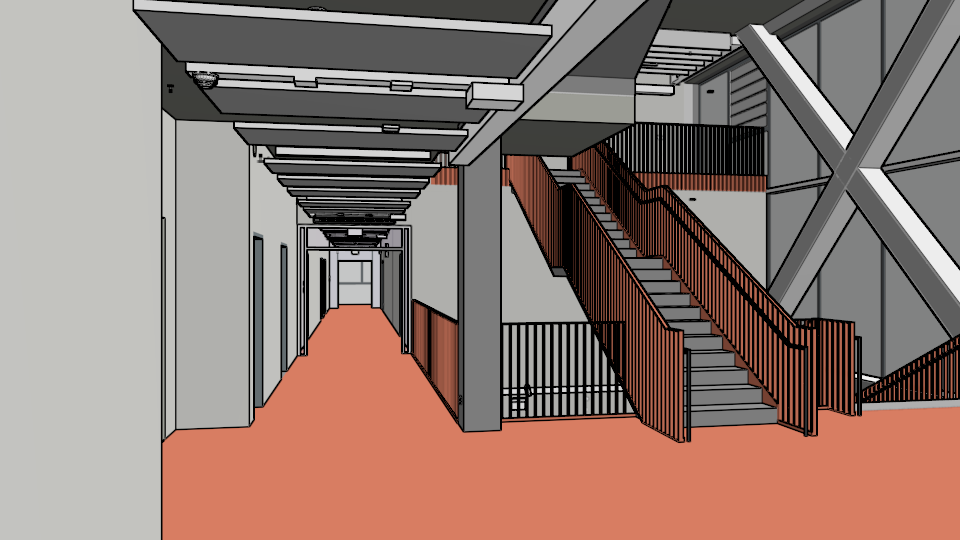
\includegraphics[width=\linewidth]{images/syn_dataset/hs_gamma02162.png}
		\caption{HS Simulation}
		\label{subfig:hs_gamma_syn_example}
	\end{subfigure}
	\caption{Veranschaulichung der Gebäudesimulationen. Für eine bessere Visualisierung sind die Kanten markant dargestellt. Während die Wände, die Decke und der Boden in \subref{subfig:ic_syn_example} wenig Detail beinhalten, sind diese in \subref{subfig:hs_gamma_syn_example} detailreicher mit technischen Gebäudeausrüstungen wie z.B. Steckdose ausgestattet.}
	\label{fig:difference_3d}
\end{figure} 

\begin{table}
	\centering
	\caption{Approximierte metrische Eigenschaften der Datensätze.}
	\begin{tabularx}{1.0\textwidth}{X X X >{\centering\arraybackslash}p{1.7cm} }
		\textbf{Bezeichnung} & \textbf{Streckenlänge} & \textbf{Volumen} & \textbf{Gebäude}\\
		\hline
		IC-loop & $115m$ & $50m \times 11m \times 3.5m$ & IC \\
		\hline
		HS-gamma & $65m$ & $54m \times 10m \times 3m$ & HS\\
		\hline
		HS-stairs-up & $32m$ & $12m \times 12m \times 12m$ & HS\\
		\hline
		HS-stairs-down & $32m$ & $12m \times 12m \times 12m$ & HS\\
	\end{tabularx}
	\label{tab:dataset_metrics}
\end{table}


\begin{table}
	\centering
	\caption{Datenmenge der Datensätze.}
	\begin{tabularx}{1.0\textwidth}{p{3.5cm} X  >{\centering\arraybackslash}p{1.7cm} }
		\textbf{Bezeichnung} & \textbf{Anzahl reale Daten} (synthetische Daten) & \textbf{Gebäude}\\
		\hline
		IC-loop & 3842 (11435) & IC\\
		\hline
		HS-gamma & 1958 (6490) & HS\\
		\hline
		HS-stairs-up  & 1068 (3160)& HS\\
		\hline
		HS-stairs-down & 1161 (3245) & HS\\
	\end{tabularx}
	\label{tab:datasets}
\end{table}


\begin{figure}
	\centering
	\begin{subfigure}[t]{1.0\linewidth}
		\centering
		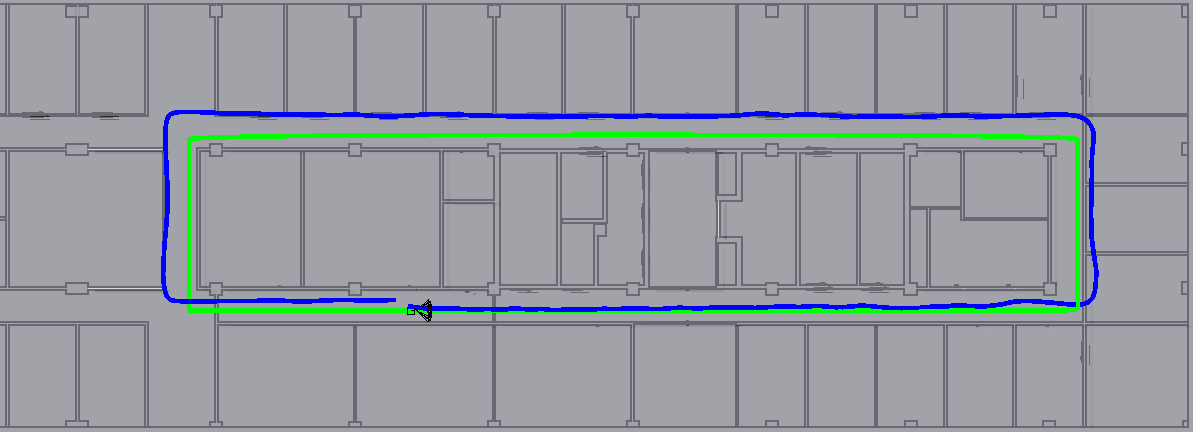
\includegraphics[width=\linewidth]{images/trajectories/ic_traj.png}
		\caption{\textit{IC-loop}}
		\label{subfig:traj_ic}
	\end{subfigure}
	\hfill \medskip
	\begin{subfigure}[t]{1.0\linewidth}
		\centering
		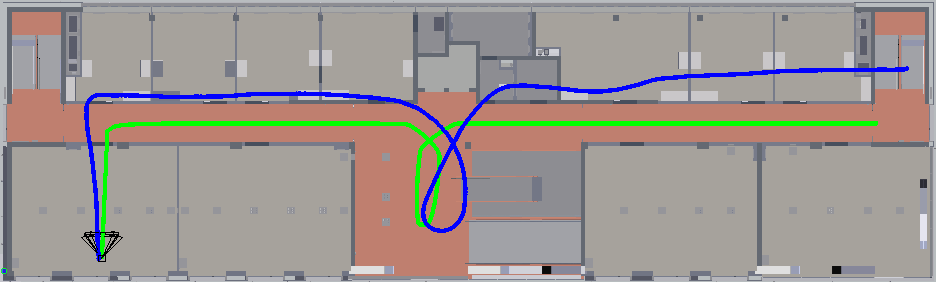
\includegraphics[width=\linewidth]{images/trajectories/hs_gamma.png}
		\caption{\textit{HS-gamma}}
		\label{subfig:traj_hs_gamma}
	\end{subfigure}
	\hfill \medskip
	\begin{subfigure}[tr]{0.45\linewidth}
		\flushleft
		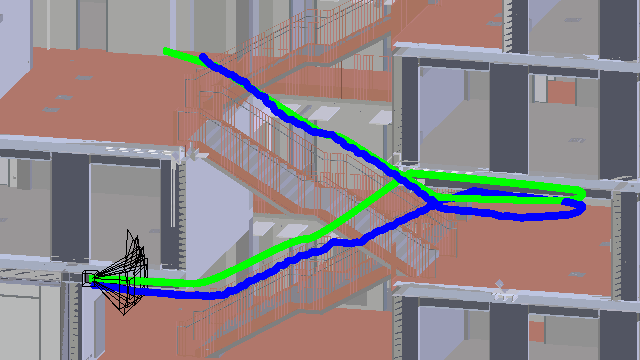
\includegraphics[width=\linewidth]{images/trajectories/hs_up.png}
		\caption{\textit{HS-stairs-up}}
		\label{subfig:traj_hs-up}
	\end{subfigure}
	\hfill
	\begin{subfigure}[tl]{0.45\linewidth}
		\flushright		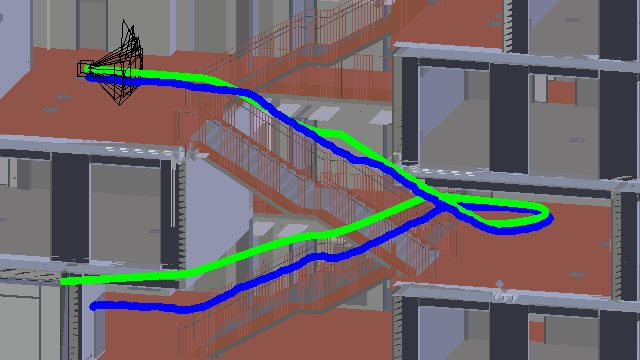
\includegraphics[width=\linewidth]{images/trajectories/hs_down.png}
		\caption{\textit{HS-stairs-down}}
		\label{subfig:traj_hs-down}
	\end{subfigure}
	\hfill
	\caption{Illustration der Aufnahmestrecken der Datensätze. Die Aufnahmestrecken der synthetischen Daten werden in Grün und die, von der T265 mit einer Abweichung bis zur 5\% berechneten, Strecke der realen Daten in Blau gekennzeichnet. \subref{subfig:traj_ic} befindet sich in der nördlichen Hälfte des 6. Stockwerkes des IC-Gebäudes Ruhr-Universität Bochum. \subref{subfig:traj_hs_gamma}, \subref{subfig:traj_hs-up}, \subref{subfig:traj_hs-down} befinden sich im Seminargebäude Hochschule Bochum. \subref{subfig:traj_hs-up} und \subref{subfig:traj_hs-down} sind nahe an der Position der Schleife von \subref{subfig:traj_hs_gamma}. Tabelle \ref{tab:dataset_metrics} listet die approximierten metrischen Eigenschaften der Aufnahmestrecken auf.}
	\label{fig:trajectories}
\end{figure}

\subsection{Trainingsparameter}
Künstlichen neuronalen Netzwerke (\textit{KNN}) besitzen zwei Arten von Parametern. Die erste Art von Parametern (\textit{Gewichte}) werden während der Trainingsphase über \textit{Backpropagation}-Verfahren an die Trainingsdaten angepasst.
Die zweite Art von Parametern (\textit{Hyperparameter}) werden vor der Trainingsphase festgelegt und geben besondere Einstellungen des Netzwerkes wie z.B. das Lernverhalten an. Die Performance eines KNNs ist abhängig von seinen Parametern \cite{Goodfellow-et-al-2016}. Da diese Arbeit den Ansatz von \citet{acharyaBIMPoseNetIndoorCamera2019} auf längeren Strecken in größeren Gebäudesimulation zu untersuchen versucht, wurde die Performance des KKNs bestmöglich von den verwendeten Datensätzen abhängig gehalten, indem die Hyperparametern von \citet{acharyaBIMPoseNetIndoorCamera2019} übernommen bzw. gleichermaßen bestimmt oder im selben Verhältnis zur Datensatz gewählt wurden.

% Hyperparameter können über Grid-Search Verfahren optimiert werden, indem die Akkuratesse der Netzwerke mit variierenden Hyperparametern paarweise verglichen werden


In der vorliegenden Arbeit wurde für das Training des Netzwerkes die Caffe \cite{jiaCaffeConvolutionalArchitecture2014} Implementierung von PoseNet verwendet, die von den eigenen Autoren \citet{kendallPoseNetConvolutionalNetwork2015} veröffentlicht wurde. Die Batchgröße betrug 40 und die Anzahl der Trainingsepochen war 160. Eine NVIDIA GeForce GTX 1080 Ti mit 11GB Grafikspeicher wurde verwendet und ermöglichte bei einer Batchgröße von 40 drei Trainingsprozesse zeitgleich durchzuführen.

Der Hyperparameter $\beta$, der von PoseNet vorgestellten Kostenfunktion (vgl. Gleichung \ref{eq:posenet_loss}), wurde wie empfohlen für jeden realen Datensatz durch ein Grid-Search Verfahren bestimmt, indem mit der zufällig angeordneten Hälfte der realen Daten trainiert und mit der restlichen Hälfte evaluiert wurde. Der Loss wurde mit dem AdaGrad \cite{duchiAdaptiveSubgradientMethods2011} Gradientenabstiegsverfahren mit einer konstanten Lernrate von $10^{-3}$ optimiert bzw. minimiert. 

Die Trainings- sowie Evaluationsdaten wurden auf eine Auflösung von $480\times270$ skaliert. Während des Trainingsprozesses wurden zufällige Ausschnitte der Größe $224 \times 224$ aus dem skalierten Datensatz genommen und für die Evaluierung wurde ein zentrierter Ausschnitt derselben Größe aus dem skalierten Evaluationsdatensatz verwendet. Das Durchschnittsbild der synthetischen Daten wurden beim Trainieren und bei der Evaluierung von den Inputbildern subtrahiert. 
Die Gewichte des Netzwerks wurden mit den Gewichten eines Modells initialisiert, das auf der GoogLeNet Architektur mit dem Places Datensatz trainiert wurde. Anschließend wurden die Gewichte an die Trainingsdaten angepasst. Tabelle \ref{tab:trainingparams} gibt eine Übersicht der Hyperparameter an.

\cleardoublepage
\begin{table}[bp]
	\centering
	\caption{Übersicht der Hyperparameter.}
	\begin{tabularx}{1.0\textwidth}{X X}
		\textbf{Hyperparameter} & \textbf{Wert}\\
		\hline
		Architektur & PoseNet (siehe Abschnitt \ref{sec:posenet})\\
		\hline
		Implementierung & Caffe \cite{jiaCaffeConvolutionalArchitecture2014} \\
		\hline
		Batchgröße & $40$\\
		\hline
		Anzahl der Epochen & $160$\\
		\hline
		\makecell[tl]{
			$\beta$ der Kostenfunktion\\
			(siehe Gleichung \ref{eq:posenet_loss}) 
		} &
		\makecell[tl]{
			IC-loop: 680\\
			HS-gamma: 120\\
			HS-stairs-up 470\\
			HS-stairs-down: 610\\
		}\\
		\hline
		Loss-Optimierer & AdaGrad\\
		\hline
		Lernrate & $10^{-3}$\\
		\hline
		Bildskalierung & $480 \times 270$\\
		\hline
		Bildausschnitt& \makecell[tl]{
			$224 \times 244$\\
			(Training: zufällig, Evaluation: zentriert)\\
		}\\
		\hline
		Datensatznormierung & Subtraktion des Durchschnittsbildes der synthetischen Daten \\
		\hline
		Initialisierung der Gewichte & Gewichte eines mit dem Places Datensatz trainierten Modells auf GoogLeNet \\
	\end{tabularx}
	\label{tab:trainingparams}
\end{table}
\cleardoublepage